\documentclass[10.5pt]{jarticle}

\usepackage{kws}
%%%%%%%% added by Keito Murata %%%%%%%%%%%%%%%
\usepackage{setspace}
\usepackage{bm}
\usepackage[dvipdfmx]{color}
\usepackage[dvipdfmx]{graphicx}
\usepackage{amsmath}
\usepackage{amssymb}
\usepackage{amsfonts}
\usepackage{relsize}
\usepackage{url}
\usepackage{algorithm}
\usepackage{algorithmic}
\usepackage{tabularx}
\usepackage{array}
\usepackage{subcaption}
\usepackage{comment}
\newcommand{\nr}{\mathbb{R}_{\geq 0}}
\newcommand{\nc}{\mathbb{C}}
\newcommand{\nN}{\mathbb{N}}
\newcommand{\nrindex}{\mathbb{R}_{\scalebox{0.5}{$[0,1]$}}}
\newcommand{\lsum}{\mathsmaller{\sum}}
\renewcommand{\figurename}{Fig.}
\renewcommand{\tablename}{Table}
\renewcommand{\footnotesize}{\scriptsize}
%%%%%%%% added by Keito Murata %%%%%%%%%%%%%%%

\begin{document}
%
% もし、本文が英文ならば、日本語のタイトルと著者は不要です。
% その場合、下記の\OnlyEnglishtrueを有効にしてください。
% 英語のタイトルと著者のみを表示します。
% ただし、\jtitle, \jauthor, \jaddressの行は削字しないでください。
%\OnlyEnglishtrue


\jtitle{レーダセンサ及びブラインド信号源分離に基づく心拍推定}

\etitle{Heart Rate Estimation Based on Radar Sensor and Blind Source Separation}

\jauthor{村田佳斗$^{\dag}$ \hspace{0.5cm} 北村大地$^{\dag}$ \hspace{0.5cm} 斎藤諒$^{\ddag}$ \hspace{0.5cm} 植木大地$^{\ddag}$ \hspace{0.5cm} 石原尚$^{\ddag}$ \hspace{0.5cm} 市ノ瀬吏$^{\ddag}$}

\eauthor{Keito Murata$^{\dag}$ \hspace{0.1cm} Daichi Kitamura$^{\dag}$ \hspace{0.1cm} Ryo Saito$^{\ddag}$ \hspace{0.1cm} Daichi Ueki$^{\ddag}$ \hspace{0.1cm} Takashi Ishihara$^{\ddag}$ \hspace{0.1cm} Tsukasa Ichinose$^{\ddag}$}

\jaddress{\dag 香川高等専門学校 \\ \ddag 株式会社村田製作所}

\eaddress{\dag National Institute of Technology, Kagawa College \\ \ddag Murata Manufacturing Co., Ltd.}


\maketitle

%%%%%%%% added by Keito Murata %%%%%%%%%%%%%%%
\setlength{\abovedisplayskip}{4pt}
\setlength{\belowdisplayskip}{4pt}
\renewcommand{\thefootnote}{\arabic{footnote}}
%%%%%%%% added by Keito Murata %%%%%%%%%%%%%%%

%----------------------------------------------
\section{はじめに}
%----------------------------------------------

\hspace{1em}自動車の運転中に運転者が睡眠,突発的な発作,体調の悪化による意識喪失等に見舞われることは多くの場合致命的な状況となる.そのため,運転中に運転者の状態を何らかの方法で管理することが重要課題の一つとなっている.

この課題に取り組むために,本稿では,Fig.~\ref{fig:sensorstructure}に示す運転中の運転者の心拍をレーダ非接触型生体センサアレイ(以後,レーダセンサと呼ぶ)を活用した常時モニタリングシステム(以後,振動測定系と呼ぶ)を取り扱う.この振動測定系においては,目的としている心拍信号以外にも振動測定系自体のノイズ,運転者の体動,呼吸による体表面変動等の信号も同時に観測されるため,信号対ノイズ比(signal-to-noise ratio: SNR)を著しく低下する.本稿の目的は,観測信号が低SNRとなる問題に対してブラインド信号源分離(blind source separation: BSS)\cite{originica}において代表的な手法である独立ベクトル分析(independent vector analysis: IVA\cite{Kim2007_iva, auxIVA})及び独立低ランク行列分析(independent low-rank matrix analysis: ILRMA\cite{ILRMA, Kitamura2018_ilrma})を適用することで,心拍の推定精度の向上を目指すことである.本稿で仮定する状況では,レーダセンサや体表面の位置関係が事前に未知であるため,心拍信号の分離にBSSを適用することは妥当と考えられる.また,心拍推定アルゴリズムを適用して心拍推定を行い心拍推定精度についても同様に検討を行う.

%-%-%-%-%-%-%-%-%
\begin{figure}[tb]
  \centering
  \vspace{0pt} % 図上部の余白調整
  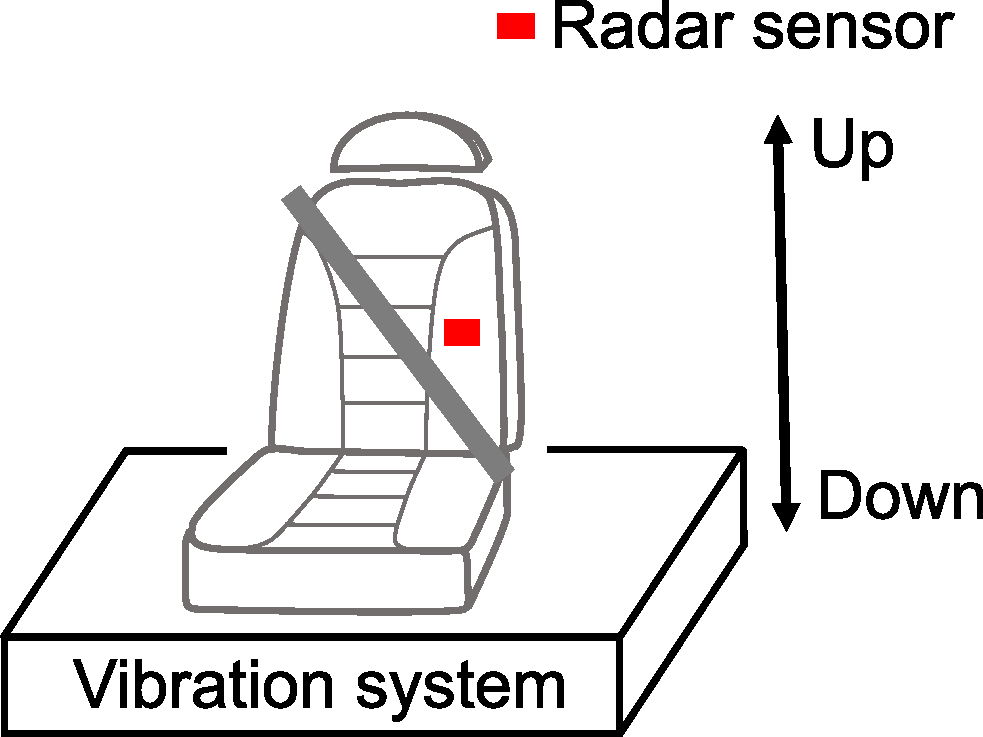
\includegraphics[width=0.6\columnwidth]{sensorstructure.pdf}
  \vspace{0pt} % 図とキャプション間の余白調整
  \caption{Vibration measurement system and driver's seat with radar sensor.}
  \vspace{-10pt} % キャプション下部の余白調整
  \label{fig:sensorstructure}
\end{figure}
%-%-%-%-%-%-%-%-%

%-%-%-%-%-%-%-%-%
\begin{figure}[tb]
  \centering
  \vspace{0pt} % 図上部の余白調整
  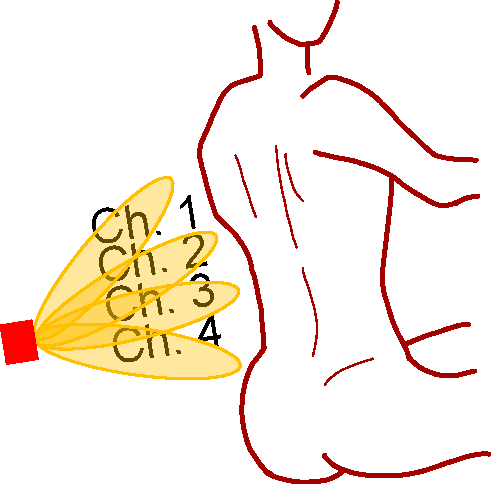
\includegraphics[width=0.4\columnwidth]{sensorimg.pdf}
  \vspace{0pt} % 図とキャプション間の余白調整
  \caption{Beams from radar sensor for measurering back of driver's body.}
  \vspace{-20pt} % キャプション下部の余白調整
  \label{fig:sensorimg}
\end{figure}
%-%-%-%-%-%-%-%-%

%----------------------------------------------
\section{振動測定系と測定条件}
%----------------------------------------------
%----------------------------------------------
\subsection{振動測定系}
%----------------------------------------------

\hspace{1.0em}本稿で仮定するレーダセンサの振動測定系はFig.~\ref{fig:sensorstructure}を示す.運転者を模した被験者が座った状態で振動測定系全体を上下方向に振動させる.Fig.~\ref{fig:sensorimg}に示す通り,レーダセンサを背部にあたるシートの内部に埋め込んでいるため,運転者の背部の体表面の微小変位を測定することが可能である.またFig.~\ref{fig:sensorimg}に示すように,4チャネルの異なる指向性レーダで駆動しているため,同時に近傍4点の体表面変位を測定した4~chの観測信号を得ることができる.

%----------------------------------------------
\subsection{レーダセンサの観測スペクトログラム}
%----------------------------------------------

\hspace{1.0em}レーダセンサで観測された信号の内1~chのスペクトログラムをFig.~\ref{fig:1chobs}に示す.観測信号には心拍以外にも,振動台による振動成分及び呼吸に起因する体動成分等が混在していることが確認できる.そのため,本稿ではBSSを用いて心拍成分のみを抽出することを目指す.

また本稿では,分離した信号と比較する参照値を得るために,Zephyr Technology社の接触型心電図センサ(ECG)Bioharnessを用いてECG信号を取得している.心拍の参照値の計算には,このBioharness内部で実装されているアルゴリズムを用いる.Bioharnessの技術的な資料は公開されておらず原理は不明であるが,恐らく一般的な心拍推定アルゴリズムであるR-R間隔(R波と呼ばれる心拍波形の間隔)推定に基づくものと予想される.また,このECGセンサのサンプリング周波数は250~Hzである.接触型ECGセンサであるため,振動台の振動が加えられても高精度な心拍を得ることが可能である.本稿では,このECGセンサから得られる心拍と同程度の精度でレーダセンサの信号から心拍を推定することが目的となる.

%-%-%-%-%-%-%-%-%
\begin{figure}[tb]
  \centering
  \vspace{0pt} % 図上部の余白調整
  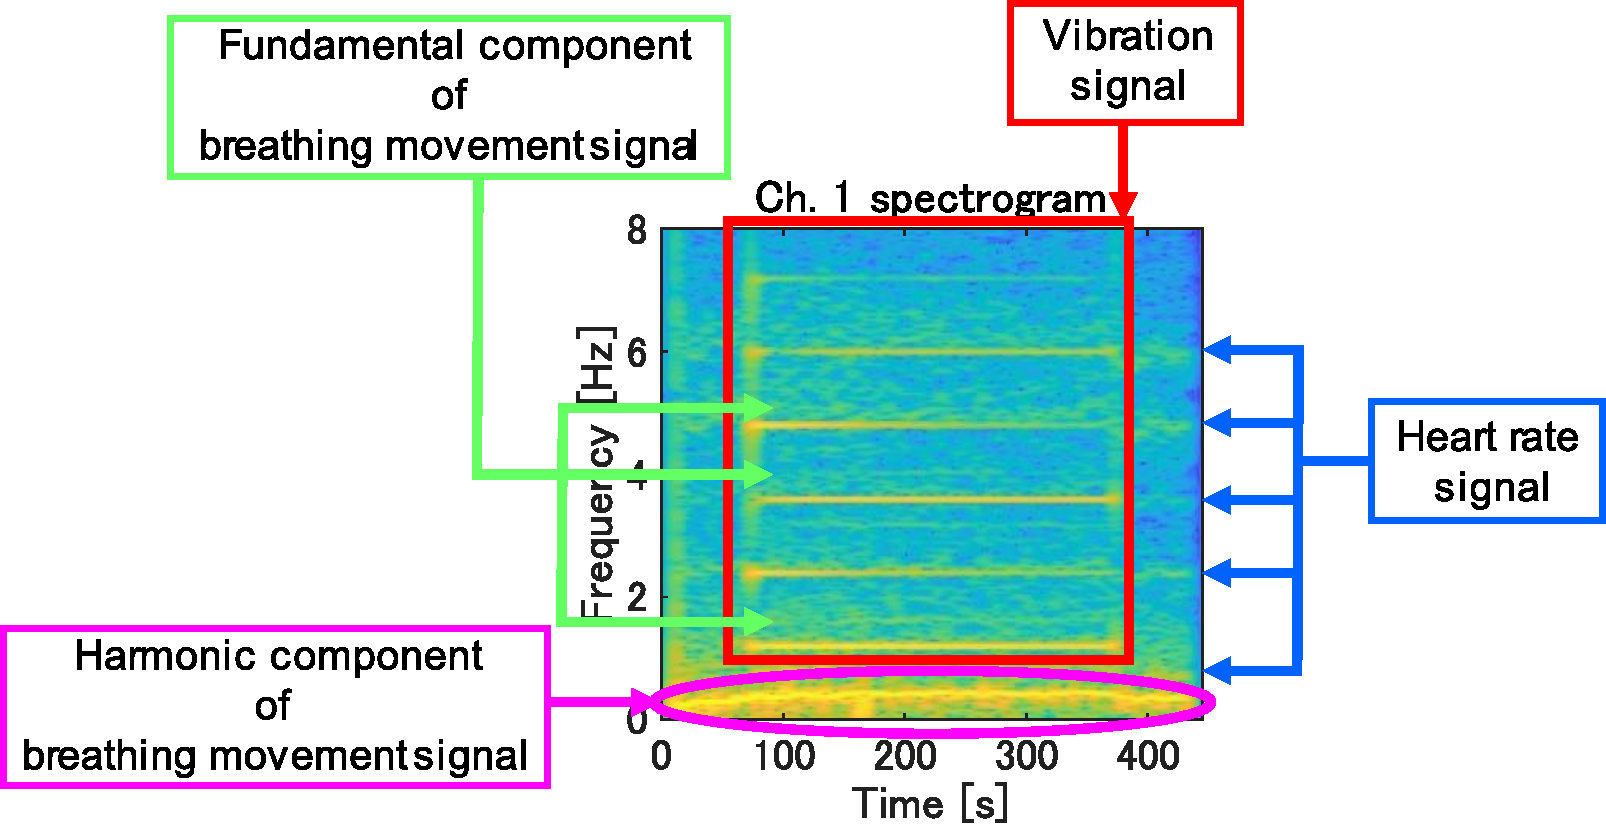
\includegraphics[width=1.0\columnwidth]{1chobsspect.pdf}
  \vspace{-20pt} % 図とキャプション間の余白調整
  \caption{Each component in first channel spectrogram obtained by radar sensor.}
  \vspace{-20pt} % キャプション下部の余白調整
  \label{fig:1chobs}
\end{figure}
%-%-%-%-%-%-%-%-%

%----------------------------------------------
\section{BSS及び心拍推定アルゴリズム}
%----------------------------------------------
%----------------------------------------------
\subsection{BSSの定式化}
%----------------------------------------------

\hspace{1.0em}以下に,時間周波数領域BSSの定式化を行う.
信号源$( \tilde{\bm{s}}[l] )_{l=1}^L$,観測信号$( \tilde{\bm{x}}[l] )_{l=1}^L$,及び分離信号$( \tilde{\bm{y}}[l] )_{l=1}^L$のそれぞれに対して{STFTを適用したものを次式で定義する.}
\begin{align}
\bm{s}_{ij} &= [s_{ij1}, s_{ij2}, \cdots, s_{ijn}, \cdots, s_{ijN}]^{\mathrm{T}} \in \mathbb{C}^{N} \label{eq:s} \\
\bm{x}_{ij} &= [x_{ij1}, x_{ij2}, \cdots, x_{ijm}, \cdots, x_{ijM}]^{\mathrm{T}} \in \mathbb{C}^{M} \label{eq:x} \\
\bm{y}_{ij} &= [y_{ij1}, y_{ij2}, \cdots, y_{ijn}, \cdots, y_{ijN}]^{\mathrm{T}} \in \mathbb{C}^{N} \label{eq:y}
\end{align}
ここで,$i=1, 2,  \cdots, I$及び$j=1, 2,  \cdots, J$はそれぞれ周波数ビンインデクス及び時間フレームインデクスを表す.また,式\eqref{eq:s}--\eqref{eq:y}の各信号においては,時間周波数行列としての表記もそれぞれ$\bm{S}_n\in\mathbb{C}^{{I\times J}}$,$\bm{X}_m\in\mathbb{C}^{{I\times J}}$,及び$\bm{Y}_n\in\mathbb{C}^{{I\times J}}$として定義しておく.
{式(\ref{eq:s})--(\ref{eq:y})において},周波数毎の時不変な(時間フレーム$j$に依存しない)瞬時混合は,混合行列$\bm{A}_i \in \mathbb{C}^{M\times N}$を用いて次式で表せる.
\begin{align}
  \bm{x}_{ij} = \bm{A}_i \bm{s}_{ij} \label{eq:xas}
\end{align}
時間領域の場合と同様に$M=N$かつ$\bm{A}_i$がフルランクの場合は,分離行列$\bm{W}_{i} = [\bm{w}_{i1}~\bm{w}_{i2}~\cdots~ ~\bm{w}_{iN}]^{\mathrm{H}} \in \mathbb{C}^{N \times M} $が存在し,分離信号は次式で表せる.
\begin{align}
  \bm{y}_{ij} = \bm{W}_i \bm{x}_{ij} \label{eq:ywj}
\end{align}
ここで,$^{\mathrm{H}}$は行列及びベクトルのエルミート転置を表す.従って,
{時間周波数領域BSSは周波数毎の混合行列$\bm{A}_i$が未知の状態で周波数毎の分離行列$\bm{W}_{i} \approx \bm{A}_i^{-1}$}を全ての周波数$i=1, 2, \cdots, I$において推定する問題である.但し,そのままでは周波数毎に分離された信号源の順序($\bm{y}_{ij}$のベクトルの要素の順序)が周波数間で統一されない問題が生じる.これは時間周波数領域BSSにおけるパーミュテーション問題\cite{permute}と呼ばれ,これまで様々な解決法が提案されてきた(例えば\cite{persolve1,persolve2,persolve3,persolve4}等).近年では,信号源間の統計的独立性だけでなく,各信号源の時間周波数表現に何らかの構造を仮定することで,パーミュテーション問題を回避するBSSが主流となっている.特に,次節以降で述べるIVA及びILRMAが良く用いられる代表的な時間周波数領域
BSSとなっている.

%----------------------------------------------
\subsection{IVA}
%----------------------------------------------

%-%-%-%-%-%-%-%-%
\begin{figure*}[htbp]
      \begin{minipage}[t]{0.45\hsize}
        \centering
        %\vspace{0pt} % 図上部の余白調整
        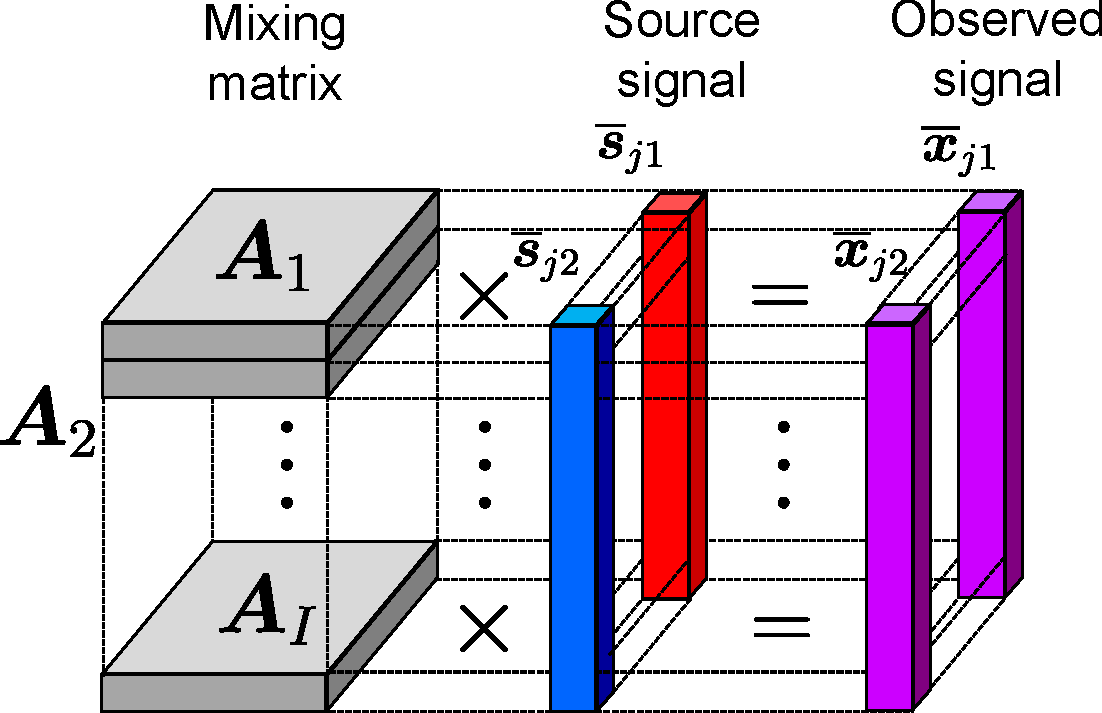
\includegraphics[keepaspectratio, width=6cm]{mixingiva.pdf}
        \subcaption{Mixing model}
        \label{fig:mixingiva}
      \end{minipage} 
      \begin{minipage}[t]{0.45\hsize}
        \centering
        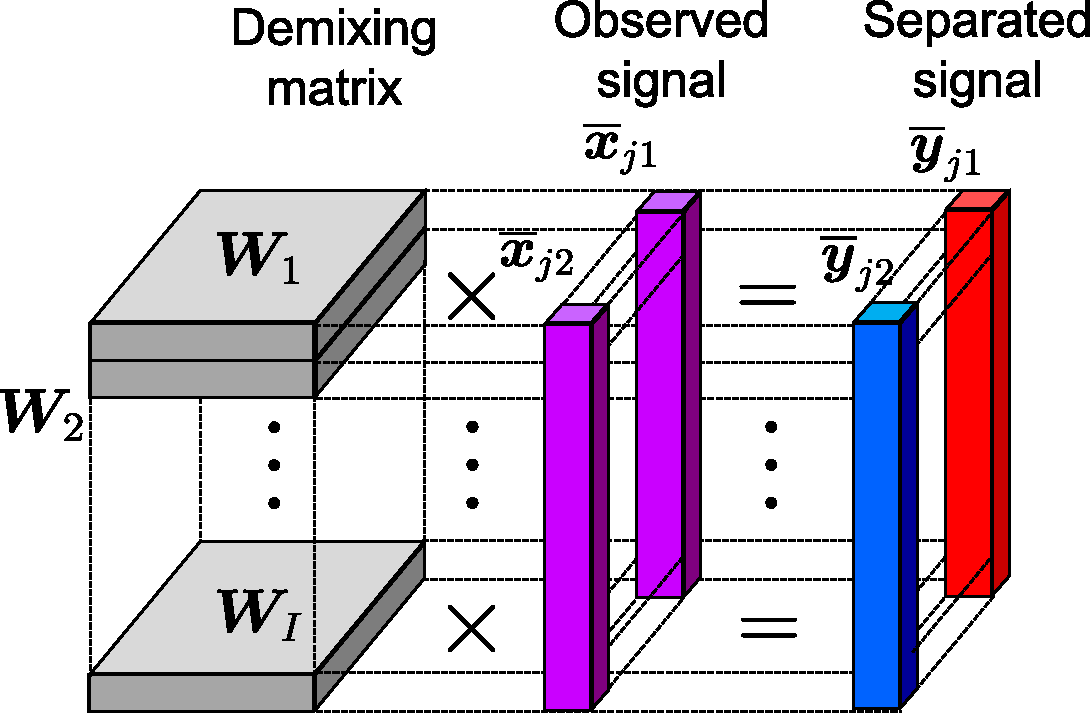
\includegraphics[keepaspectratio, width=6cm]{demixingiva.pdf}
        \subcaption{Demixing model}
        \label{fig:demixingiva}
      \end{minipage} 
     \vspace{-10pt} % 図とキャプション間の余白調整
     \caption{Mixing and demixing models assumed in IVA, where $M=N=2$.}
     \vspace{-15pt} % キャプション下部の余白調整     
     \label{fig:ivamodel}
  \end{figure*}
%-%-%-%-%-%-%-%-%

信号源,観測信号,及び分離信号のそれぞれについて,全ての周波数ビンに関する成分をまとめたベクトルを次のように定義する.
\begin{align}
    \overline{\bm{s}}_{jn} &= [s_{1jn}, s_{2jn}, \cdots, s_{ijn}, \cdots, s_{Ijn} ]^{\mathrm{T}} \in \mathbb{C}^{I} \\
    \overline{\bm{x}}_{jm} &= [x_{1jm}, x_{2jm}, \cdots, x_{ijm}, \cdots, x_{Ijm} ]^{\mathrm{T}} \in \mathbb{C}^{I} \\
    \overline{\bm{y}}_{jn} &= [y_{1jn}, y_{2jn}, \cdots, y_{ijn}, \cdots, y_{Ijn} ]^{\mathrm{T}} \in \mathbb{C}^{I}
\end{align}
Fig. \ref{fig:ivamodel}に$M=N=2$の場合におけるIVAの混合系及び分離系のモデル図を示す.
IVAは時間周波数領域BSSであるため,全周波数の分離行列$( \bm{W}_i )_{i=1}^I$を推定する.
ただし,推定の過程において,全周波数を含む$I$次元{複素}分布を各信号源{$\overline{\bm{s}}_{jn}$の生成モデルと仮定している.さらに,この}$I$次元ベクトル内には高次相関(ベクトル内の要素が共起するという性質)があることを仮定している.
このIVAの生成モデルには$I$次元球対称複素Laplace分布が用いられ,式\eqref{eq:iva_model}で表される.
\begin{align}
  \nonumber p(\overline{\bm{s}}_{jn}) &= p(\overline{\bm{y}}_{jn}) \\
&= \frac{1}{\pi \prod_{i} \sigma_{in}} \exp \left(  - \sqrt{ \sum_i \left| \frac{y_{ijn}}{\sigma_{in}} \right|^2}  \right)
\label{eq:iva_model}    
\end{align}
ここで,$\sigma_{in}>0$はスケールパラメタである.
式(\ref{eq:iva_model})の分布は球対称性を持つため,同一ベクトル内の成分が高次相関を持つ\cite{Kim2007_iva}.
したがって,IVAは同時に生起する周波数成分を一つの信号源としてまとめる傾向がある.この性質は,信号源が基本周波数成分とその整数倍の周波数成分からなる場合(調波構造を持つ場合)に,それらの成分を同一の信号源の成分とみなすことに対応する.そして,そのような信号源が出力されるように分離行列$( \bm{W}_i )_{i=1}^I$が推定される.即ち,もし各信号源が実際に周波数方向の共起性を持っていれば,IVAはパーミュテーション問題を回避しながら分離行列$( \bm{W}_i )_{i=1}^I$を推定することができ,BSSが達成される.
信号源周波数ベクトル間の独立性$p(\overline{\bm{y}}_{j1}, \overline{\bm{y}}_{j2}, \cdots, \overline{\bm{y}}_{jN}) = \prod_n p(\overline{\bm{y}}_{in})$を仮定すると,IVAの観測信号に対する負対数尤度関数は次式で得られる.
\begin{align}
    \mathcal{L} = -2J \sum_i \log |\det \bm{W}_i| + \sum_{j,n} G(\overline{\bm{y}}_{jn})
    \label{eq:ivalike}
\end{align}
ここで,$G(\overline{\bm{y}}_{jn})$はコントラスト関数と呼ばれ,次式で定義される.
\begin{align}
  \nonumber G(\overline{\bm{y}}_{jn}) &= -\log p(\overline{\bm{y}}_{jn}) \\
  \nonumber  &= -\log \frac{1}{\pi \prod_{i} \sigma_{in}} \exp \left(  - \sqrt{ \sum_i \left| \frac{y_{ijn}}{\sigma_{in}} \right|^2}  \right) \\
  &= \log \pi + \sum_i \log \sigma_{in} + \frac{1}{2} \log \sum_i \left| \frac{y_{ijn}}{\sigma_{in}}\right|^2
\end{align}
IVAにおける分離行列$( \bm{W}_i )_{i=1}^I$の推定は,最尤推定(式\eqref{eq:ivalike}の最小化)として定式化される.この最適化問題は, 補助関数法\cite{auxfunc}{及び反復射影法(iterative projection: IP)\cite{auxIVA}を用いた最適化アルゴリズムによって,高速かつ安定に解くことができる\cite{stable_auxIVA}.この反復最適化更新則は下記の通りである.}
\begin{align}
\bm{G}_{in} &= \frac{1}{J} \sum_j \frac{1}{\sqrt{\sum_{i} |\bm{w}_{in}^\mathrm{H}\bm{x}_{ij}|^{2}}} \bm{x}_{ij} \bm{x}_{ij}^{\mathrm{H}} \label{ep:auxIVAip1} \\
\bm{w}_{in} &\leftarrow (\bm{W}_i \bm{G}_{in})^{-1} \bm{e}_n \label{ep:auxIVAip2} \\
\bm{w}_{in} &\leftarrow \bm{w}_{in} ( \bm{w}_{in}^{\mathrm{H}} \bm{G}_{in} \bm{w}_{in} )^{-\frac{1}{2}} \label{ep:auxIVAip3}
\end{align}
ここで,$\bm{e}_{n} \in \mathbb{R}^{N}_{\{ 0, 1 \}^N}$は$n$番目の要素のみが1,他要素が0のベクトルである.
{式\eqref{ep:auxIVAip1}--\eqref{ep:auxIVAip3}を反復計算して分離行列$( \bm{W}_i )_{i=1}^I$を求めることができる.なお,この反復最適化アルゴリズムは1回の更新で負対数尤度関数\eqref{eq:ivalike}の値が減少する又は変動しないこと(単調非増加)が理論的に保証されている.}

%----------------------------------------------
\subsection{ILRMA}
%----------------------------------------------

\hspace{1.0em}時間周波数領域での共変性は,板倉斎藤擬距離に基づくNMF(Itakura--Saito NMF: ISNMF)\cite{isnmf}として提案された統計的生成モデルによって効率かつ詳細に表現可能である.ILRMAでは,このISNMFに基づく音源モデルをIVAに導入し,高精度なBSSを達成している.

ILRMAの反復最適化の概要をFig. \ref{fig:ilrma_outline}に示す.
{図中の}$\bm{T}_n\in\mathbb{R}_{\geq 0}^{I\times K}$及び$\bm{V}_n\in\mathbb{R}_{\geq 0}^{K\times J}$は,$n$番目の信号源のパワースペクトログラム$|\bm{Y}_n|^{.2}$をISNMFで低ランク近似したモデル$\bm{T}_n\bm{V}_n$の基底行列及びアクティベーション行列である.
ILRMAは,IVAに\textcolor{black}{基づく}分離行列$\bm{W}_i$の反復最適化とISNMFによる分離信号源$( |\bm{Y}_n|^{.2} )_{n=1}^N$の低ランクモデリングに対応する$( \bm{T}_n\bm{V}_n )_{n=1}^N$の反復最適化が交互に行われる.
具体的には,分離行列$( \bm{W}_i )_{i=1}^I$により推定された分離信号$( |\bm{Y}_n|^{.2} )_{n=1}^N$をISNMFで非負低ランク行列としてモデル化し,得られた$( \bm{T}_n )_{n=1}^N$及び$( \bm{V}_n )_{n=1}^N$の各時間周波数成分を各音源の生成モデルの推定パラメタに用いて分離行列$( \bm{W}_i )_{i=1}^I$を再度推定する,というプロセスが反復的に行われる.
ILRMAの生成モデルはISNMFと同様に次式の複素ガウス分布が仮定されている.
\begin{align}
    y_{ijn} &= \sum_k c_{ijnk} \\
    c_{ijnk} &= \mathcal{N}_{\mathbb{C}}(c_{ijnk}; 0, t_{ikn} v_{kjn}) \label{eq:ilrma_gen}
\end{align}
\textcolor{black}{ここで,$t_{ikn}$及び$v_{kjn}$は$\bm{T}_n$及び$\bm{V}_n$の要素である.}
また,$c_{ijnk} \in \mathbb{C}$は\textcolor{black}{$i, j, k, $及び$n$に関して}互いに独立であると仮定する.
このとき,観測\textcolor{black}{信号$(\bm{X}_n)_{n=1}^N$}が与えられた場合において, $\bm{W}_i$,$\bm{T}_n$, 及び$\bm{V}_n$を最尤推定する問題を考える.
ISNMFの\textcolor{black}{生成モデルより,}
\begin{align}
    y_{ijn} \sim \mathcal{N}_{\mathbb{C}}\left(y_{ijn};  0, \sum_k t_{ikn} v_{kjn} \right) 
  \label{eq:ISNMFmodel}
\end{align}
が成り立つので,全分離信号の結合分布は次式で表される.{
\begin{align}
    \nonumber p(\bm{Y}_1, \bm{Y}_2, \cdots, \bm{Y}_N) &= \prod_n p(\bm{Y}_n) \\
\nonumber &= \prod_{n, i, j} p(y_{ijn}) \\
\nonumber &= \prod_{n, i, j} \mathcal{N}_{\mathbb{C}} \left(y_{ijn}; 0, \sum_k t_{ikn}v_{kjn} \right) \\
&= \prod_{n, i, j} \frac{1}{\pi \sum_k t_{ikn}v_{kjn}} \exp \left( -\frac{|y_{ijn}|^2}{\sum_k t_{ikn}v_{kjn}} \right) \label{eq:combineddist}
\end{align}
式(\ref{eq:combineddist})を用いて観測信号の負対数尤度関数を求めると次式となる.
\begin{align}
  \nonumber \mathcal{L}(\mathsf{W, T, V}) &= - \log p(\bm{X}_1, \bm{X}_2, \cdots, \bm{X}_M) \\
    \nonumber &= -\log \left[p(\bm{Y}_1, \bm{Y}_2, \cdots, \bm{Y}_N) \cdot \prod_{i, j} |\det \bm{W}_i|^2\right] \\
    \nonumber &= -\log \left \{ \left[\prod_n p(\bm{Y}_n) \right] \cdot \prod_{i, j} |\det \bm{W}_i|^2\right \} \\
    \nonumber &= \mathrm{const.}- 2J \sum_{i}  \log |\det \bm{W}_i| \\
    \nonumber &+ \sum_{i,j,n} \left( \frac{|y_{ij}|^2}{\sum_k t_{ikn} v_{kjn}} + \log \sum_k t_{ikn} v_{kjn}\right) \\
    \nonumber &= \mathrm{const.}-2J \sum_i \log | \det \bm{W}_i | \\
    &+ \sum_{i,j,n} \left( \frac{|\bm{w}_{in}^{\mathrm{H}}\bm{x}_{ij}|^2}{\sum_k t_{ikn}v_{kjn}} + \log \sum_k t_{ikn}v_{kjn} \right)
    \label{eq:ilrmalike2}
\end{align}
ここで,$\mathsf{W}=\{ \bm{W}_i \}_{i=1}^I$,$\mathsf{T}=\{ \bm{T}_n \}_{n=1}^N$, 及び$\mathsf{V}=\{ \bm{V}_n \}_{n=1}^N$は最適化パラメタの集合である.

式\eqref{eq:ilrmalike2}を最小化するパラメタは,以下に示す反復最適化アルゴリズムで推定される.式\eqref{eq:ilrmalike2}を最小化する$\mathsf{T}$及び$\mathsf{V}$は,次式の更新式で反復最適化できる.
\begin{align}
    t_{ikn} \leftarrow t_{ikn} \sqrt \frac{ \sum_j |\bm{w}_{in}^{\mathrm{H}}\bm{x}_{ij}|^2 v_{kjn} \left( \sum_{k'} t_{ik'n} v_{k'jn} \right)^{-2} }{ \sum_j v_{kjn} \left( \sum_{k'} t_{ik'n} v_{k'jn} \right)^{-1} } \label{eq:MUTilrma} \\
    v_{kjn} \leftarrow v_{kjn} \sqrt \frac{ \sum_i |\bm{w}_{in}^{\mathrm{H}}\bm{x}_{ij}|^2 t_{ikn} \left( \sum_{k'} t_{ik'n} v_{k'jn} \right)^{-2} }{ \sum_i t_{ikn} \left( \sum_{k'} t_{ik'n} v_{k'jn} \right)^{-1} } \label{eq:MUVilrma}
\end{align}
一方,分離行列$\bm{W}_i$に関する最適化は,分離ベクトル$\bm{w}_{in}$をIPで更新することで達成される.
\begin{align}
\bm{U}_{in} &= \frac{1}{J} \sum_j \frac{1}{\sum_{k}t_{ikn}v_{kjn}} \bm{x}_{ij} \bm{x}_{ij}^{\mathrm{H}} \label{eq:ip1} \\
\bm{w}_{in} &\leftarrow (\bm{W}_i \bm{U}_{in})^{-1} \bm{e}_n \label{eq:ip2} \\
\bm{w}_{in} &\leftarrow \bm{w}_{in} ( \bm{w}_{in}^{\mathrm{H}} \bm{U}_{in} \bm{w}_{in} )^{-\frac{1}{2}} \label{eq:ip3}
\end{align}
\textcolor{black}{これらの更新式も, IVAやISNMFと同様に,目的関数\eqref{eq:ilrmalike2}の値が単調非増加となることが保証されている.}

%----------------------------------------------
\subsection{心拍推定アルゴリズム}
%----------------------------------------------

\hspace{1.0em}本節では,レーダセンサの観測信号やBSSで推定された心拍信号等に対して適用する心拍推定アルゴリズムについて説明する.なお,本節ではBSSにより得られる推定心拍の時間領域の分離信号を処理の対象としている.この分離信号を$( \tilde{y}_\mathrm{HR}[l] )_{l=1}^L$と表記する.本論文で使用する心拍推定アルゴリズムを下記に順を追って示す.また,心拍推定アルゴリズムの処理の流れを以下にFig.~\ref{fig:hralgo}として示す.

%-%-%-%-%-%-%-%-%
\begin{figure}[tb]
\centering
\vspace{0pt} % 図上部の余白調整
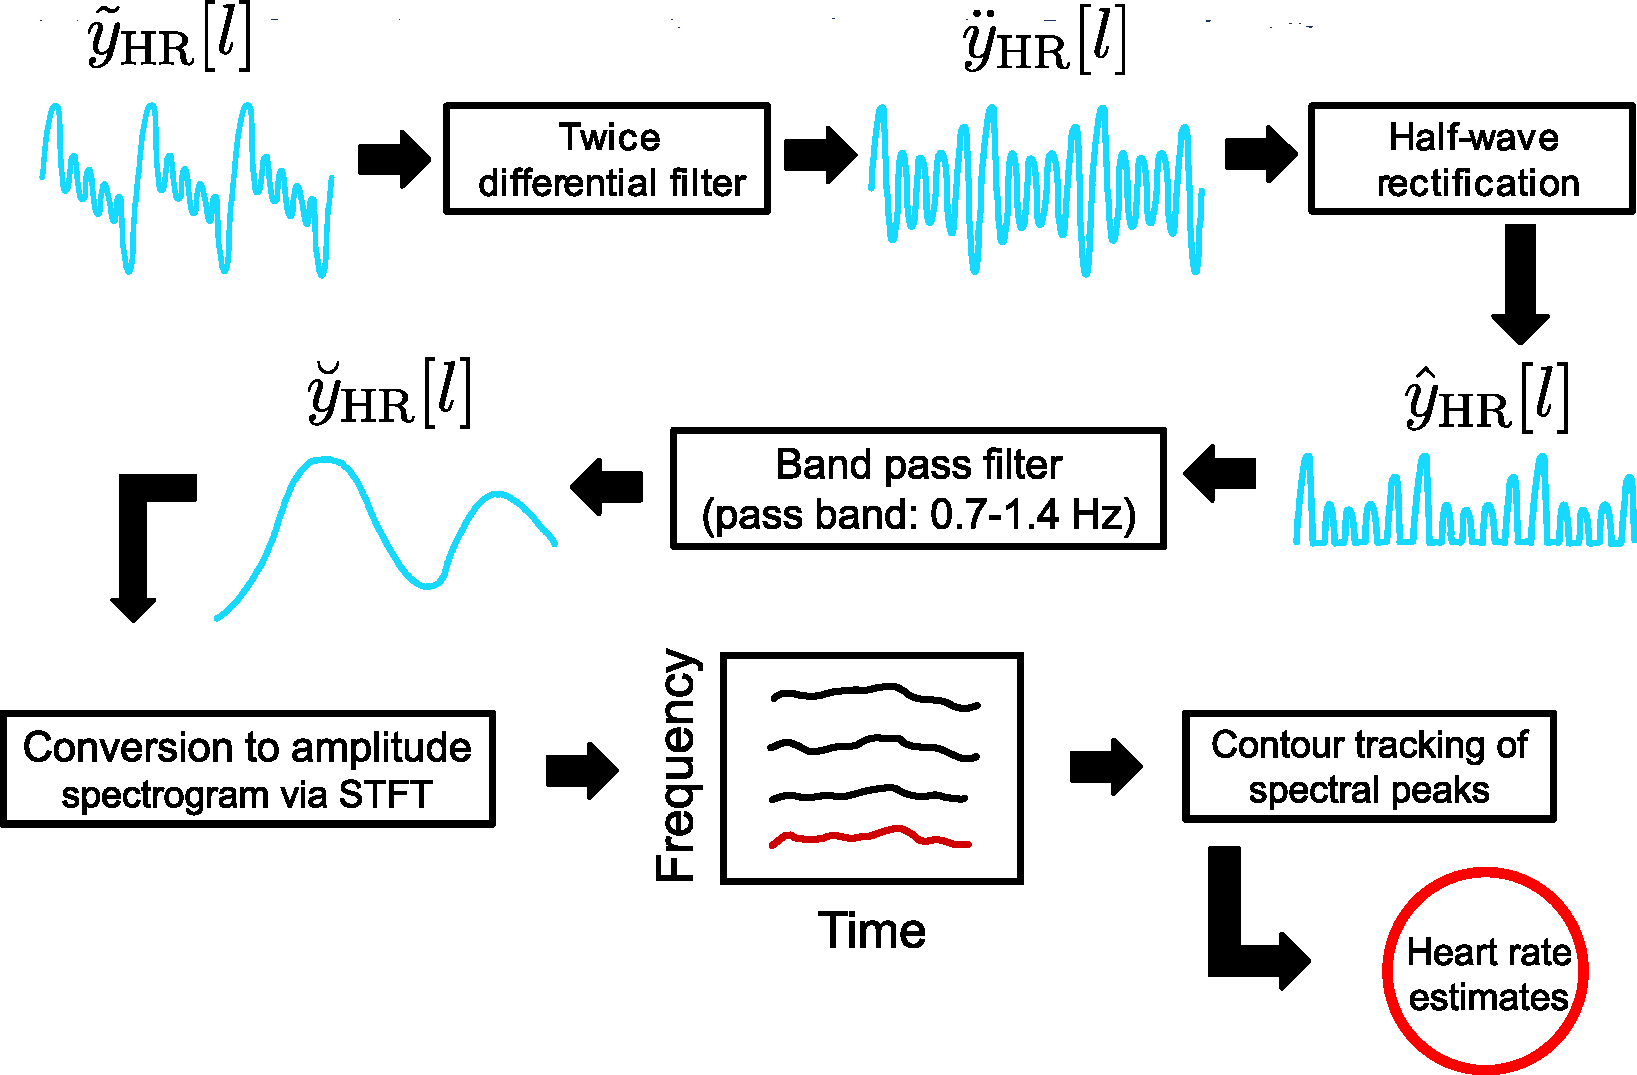
\includegraphics[width=1.0\hsize]{hralgo.pdf}
\vspace{-20pt} % 図とキャプション間の余白調整
\caption{Process of heart rate estimation algorithm.}
\vspace{-20pt} % キャプション下部の余白調整
\label{fig:hralgo}
\end{figure}
%-%-%-%-%-%-%-%-%

\textcolor{black}{まず,信号の調波構造を強調しつつ低周波成分を除去するため,次式の二階微分フィルタを信号に適用する.}
\begin{equation} 
    \begin{cases}
        \begin{split}
        & \dot{y}_\mathrm{HR}[l]=\tilde{y}_\mathrm{HR}[l+1]-\tilde{y}_\mathrm{HR}[l] \\
        & \ddot{y}_\mathrm{HR}[l]=\dot{y}_\mathrm{HR}[l+1]-\dot{y}_\mathrm{HR}[l]
        \end{split}                         &   \forall{l}
    \end{cases}
\end{equation}
次に,もう一度調波構造を強調する目的で,信号に半波整流を適用する.
\begin{equation} 
\hat{y}_{\mathrm{HR}}[l] =
    \begin{cases}
        \begin{split}
        & \ddot{y}_\mathrm{HR}[l]\quad \mathrm{if}\quad \ddot{y}_\mathrm{HR}[l]\geqq0 \\
        & 0\hspace{25pt} \mathrm{otherwise}
        \end{split}                         &   \forall{l}
    \end{cases}
\end{equation}
\textcolor{black}{さらに,心拍信号が多く存在する帯域である0.7--1.4~Hzを通過域とする5次楕円IIRバンドパスディジタルフィルタを適用する.この処理を次式で表す.}
\begin{align}
    \left(\breve{y}_{\mathrm{HR}}[l]\right)_{l=1}^{L}=\mathrm{BPF}\left[\left(\hat{y}_{\mathrm{HR}}[l]\right)_{l=1}^{L}\right]
\end{align} \label{eq:bpf}
最後に,$( \breve{y}_{\mathrm{HR}}[l] )_{l=1}^L$にSTFTを適用してスペクトログラムに変換し,振幅スペクトログラムの最大ピークとなる周波数を時間フレーム毎に求めることで,推定心拍を得る.

%----------------------------------------------
\section{観測信号にフィルタを適用しない場合のBSS及び心拍推定実験}
%----------------------------------------------
\hspace{1.0em}まず,予備実験的に観測信号に対してIVAを適用する.
%----------------------------------------------
\subsection{実験条件}
%----------------------------------------------
\hspace{1.0em}分離行列$\bm{W}_{i}$の初期値は全ての周波数に対して単位行列とした.また,IVAの式\eqref{ep:auxIVAip1}--\eqref{ep:auxIVAip3}に示した反復更新式の反復回数は100回に設定した.

%----------------------------------------------
\subsection{実験結果}
%----------------------------------------------
\hspace{1.0em}Fig. \ref{fig:siva32obs}は観測信号のスペクトログラムである.Fig.~\ref{fig:ecgspect}に接触型ECGセンサから得られる心拍信号のスペクトログラムを示す.従って,BSSで得られた分離信号の中の心拍信号がFig.~\ref{fig:ecgspect}にどの程度近いかが重要となる.これらの結果を見るとFig. \ref{fig:siva64est}では,3番目のスペクトログラムに強く心拍の高調波成分が3.5~Hz,5~Hz,及び6~Hz付近に見られる.一方で,0.4~Hz付近に呼吸による体動に起因するノイズが強く残留しており,心拍成分のみを完全に分離できていない.また,振動の高調波成分はほとんど他のスペクトログラムに分離されているが,1.2~Hzの基本周波数成分がよく残留している.1番目, 2番目, 及び4番目のスペクトログラムを見ると,3番目のスペクトログラムでは見られなかった成分が分離されているが,どれも呼吸又は振動台由来のノイズとなっている.呼吸の成分は4つの分離信号全てに残留してしまうことが多い.

%-%-%-%-%-%-%-%-%
\begin{figure}[tb]
\centering
\vspace{0pt} % 図上部の余白調整
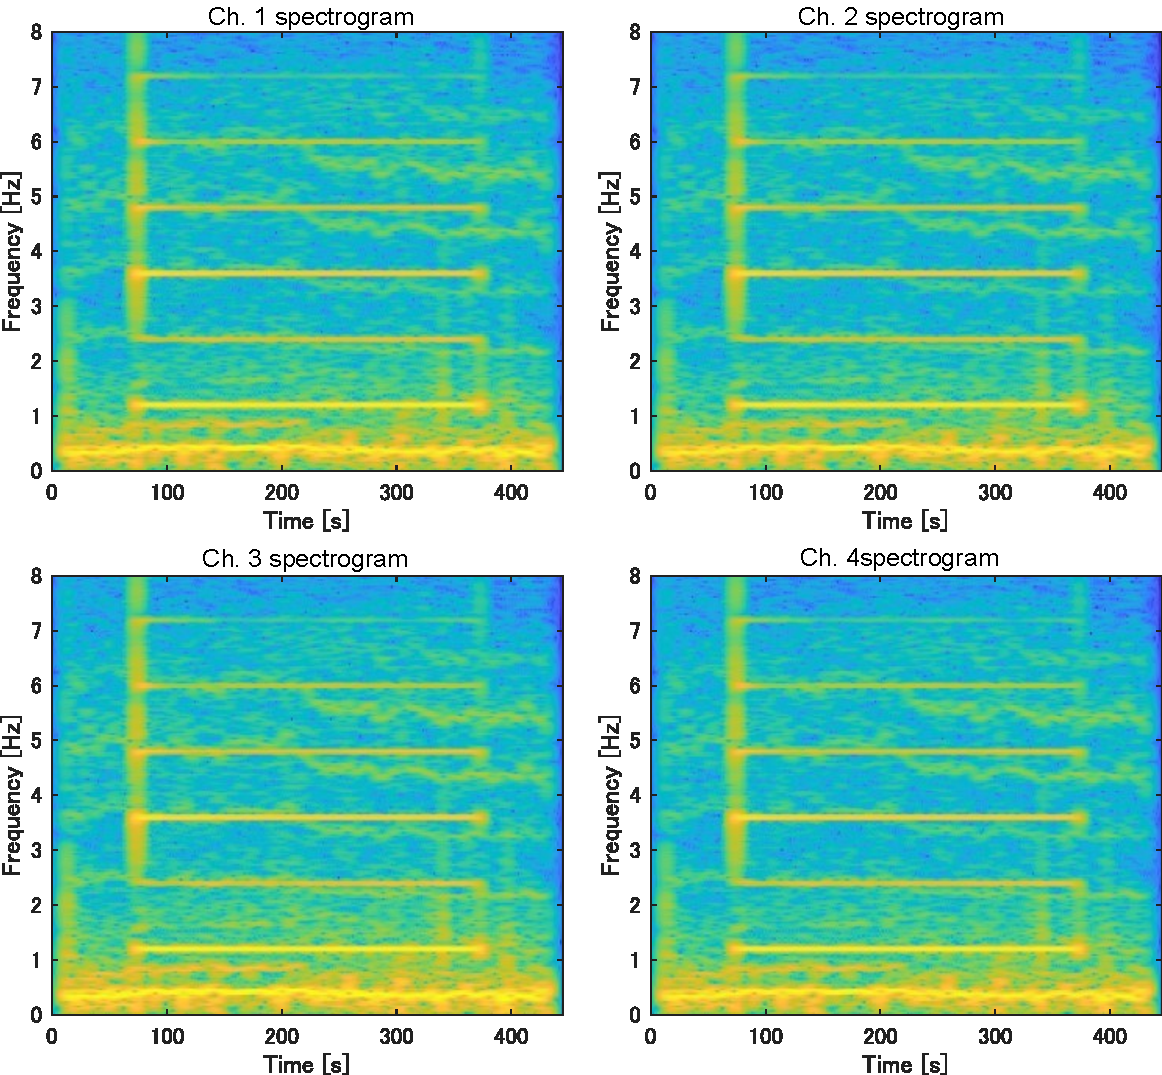
\includegraphics[width=1.0\hsize]{spect_iva_32_obs.pdf}
\vspace{-20pt} % 図とキャプション間の余白調整
\caption{Spectrograms of observed signal.}
\vspace{-20pt} % キャプション下部の余白調整
\label{fig:siva32obs}
\end{figure}
%-%-%-%-%-%-%-%-%

%-%-%-%-%-%-%-%-%
\begin{figure}[tb]
\centering
\vspace{5pt} % 図上部の余白調整
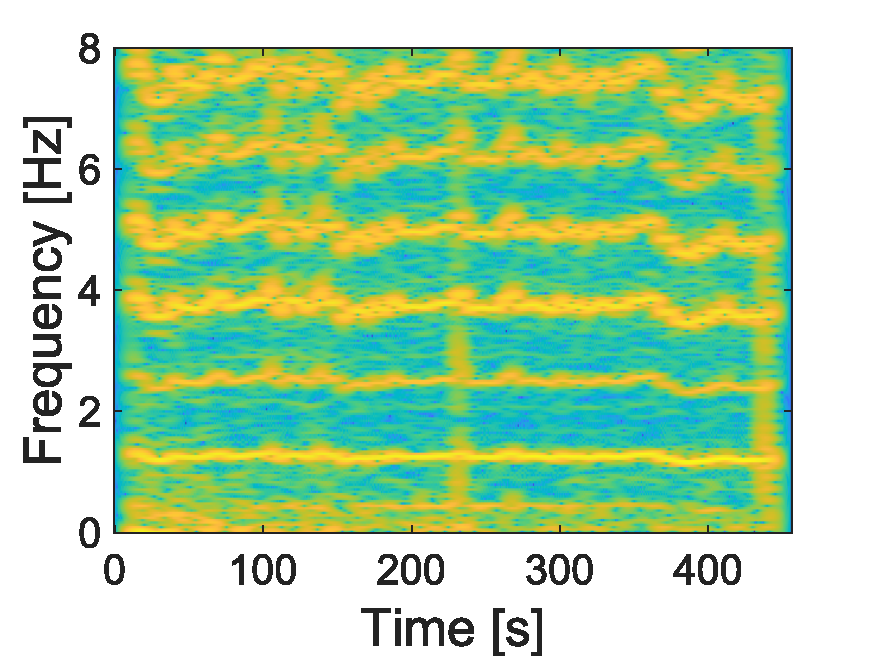
\includegraphics[width=0.7\hsize]{ecgspect.pdf}
\vspace{-10pt} % 図とキャプション間の余白調整
\caption{Spectrogram Spectrogram of observed signal obtained by contact-type ECG sensor.}
\vspace{-5pt} % キャプション下部の余白調整
\label{fig:ecgspect}
\end{figure}
%-%-%-%-%-%-%-%-%

%-%-%-%-%-%-%-%-%
\begin{figure}[tb]
\centering
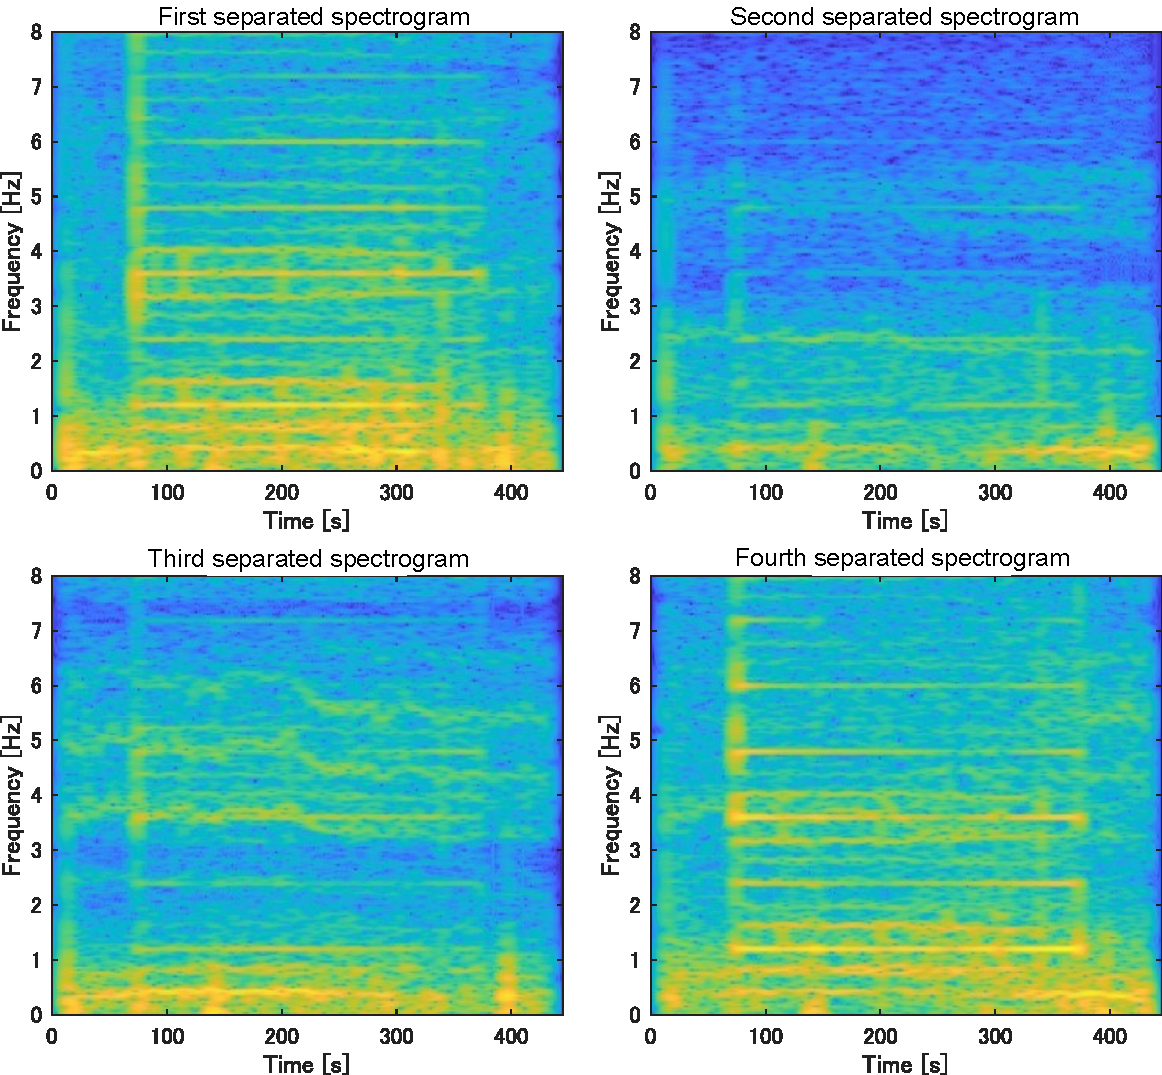
\includegraphics[width=1.0\hsize]{spect_iva_64_est.pdf}
\vspace{-20pt} % 図とキャプション間の余白調整
\caption{Spectrograms of separated signals obtained by IVA.}
\vspace{-20pt} % キャプション下部の余白調整
\label{fig:siva64est}
\end{figure}
%-%-%-%-%-%-%-%-%

%-%-%-%-%-%-%-%-%
\begin{figure}[tb]
\centering
\vspace{5pt} % 図上部の余白調整
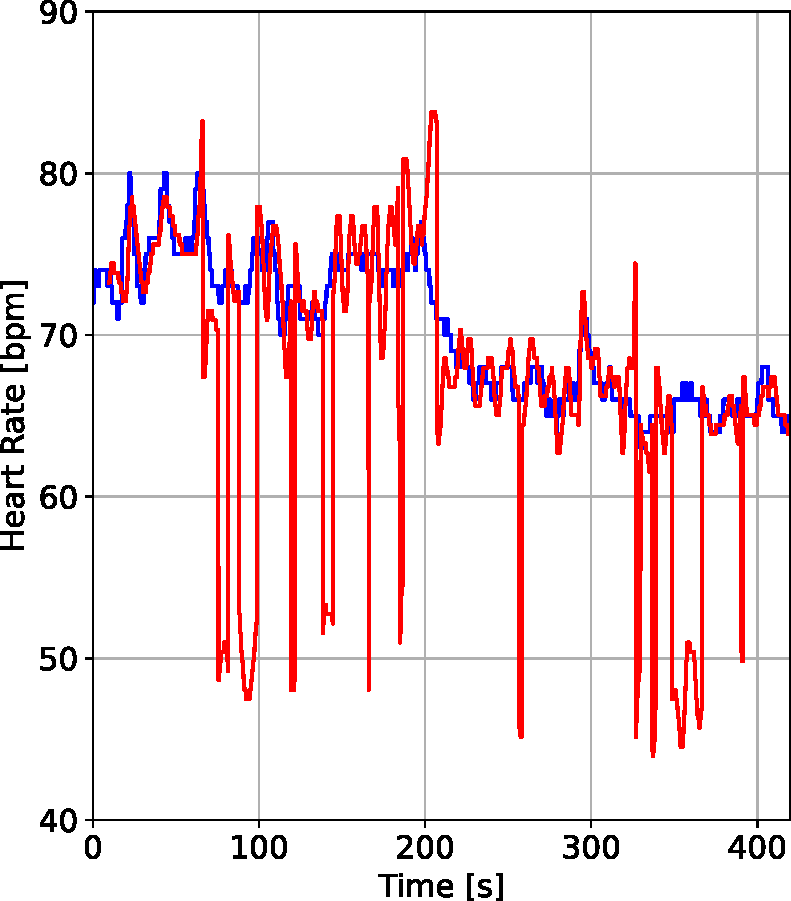
\includegraphics[keepaspectratio, width=50mm]{hr_iva_64_ch3.pdf}
\vspace{-10pt} % 図とキャプション間の余白調整
\caption{Estimated (red) and reference (blue) heart rates obtained by IVA.}
\vspace{-15pt} % キャプション下部の余白調整
\label{fig:hriva64ch3}
\end{figure}
%-%-%-%-%-%-%-%-%

%----------------------------------------------
\section{観測信号にフィルタを適用した場合のBSS及び心拍推定実験}
%----------------------------------------------
%----------------------------------------------
\subsection{前処理として適用するフィルタの設計}
%----------------------------------------------
\hspace{1.0em}観測信号のスペクトログラムであるFig.~\ref{fig:siva32obs}より,呼吸の基本周波数成分はおよそ0.4~Hz付近に存在することが確認できる.そこで,本稿では,前処理として,カットオフ周波数を1.5~Hzとするハイパスフィルタを観測信号の各チャネルに対して適用する.このハイパスフィルタは,位相歪みが生じない(線形位相特性を満たす)ようにFIRディジタルフィルタとして設計している.フィルタのタップ長(次数)は170次である.

%----------------------------------------------
\subsection{実験条件}
%----------------------------------------------
\hspace{1.0em}IVA及びILRMAのSTFTの窓長及びシフト長はそれぞれ,64点(1.6~s)及び4点(0.1~s)に設定した.IVA及びILRMAのその他の実験条件を以下に示す.

まず,IVAの実験条件を示す.分離行列$\bm{W}_{i}$の初期値は全ての周波数ビンに対して単位行列とした.また,IVAの式\eqref{ep:auxIVAip1}--\eqref{ep:auxIVAip3}に示した反復更新式の反復回数は100回に設定した.

次に,ILRMAの実験条件を示す.式\eqref{eq:ip1}--\eqref{eq:ip3}の反復更新式の反復回数は100回に設定した.また基底数を信号源毎に$K=3$とし,反復毎にプロジェクションバックで正規化を行う.基底行列及びアクティベーション行列の初期値は,区間$(0,1)$の一様乱数に設定した.

%----------------------------------------------
\subsection{実験結果}
%----------------------------------------------
%----------------------------------------------
\subsubsection{IVAを適用した結果}
%----------------------------------------------
\hspace{1.0em}Fig. \ref{fig:sfiva64est}はフィルタを適用した観測信号ににIVAを適用した結果である.
振動の3次高調波がほとんど見られず,心拍の高調波が3.5~Hz,5~Hz,及び6~Hz付近に強く現れている.1番目,2番目,及び4番目のスペクトログラムには心拍の高調波成分が見られず,振動及び呼吸の高調波成分が分離されていることが分かる.}

また,Fig. \ref{fig:sfiva64est}に対して心拍推定アルゴリズムを適用した心拍推定値をFig. \ref{fig:fhriva64ch3}に示す.前章のFig.~\ref{fig:hriva64ch3}の150~sから360~sでは合致していなかった参照値と合致していることが分かる.但し,200~s付近の推定心拍値は参照値と合致していない.この結果より,前処理を適用することで心拍推定精度が向上するといえる.しかし,加振時に参照値と合致していない箇所がまだ多く存在する.

%-%-%-%-%-%-%-%-%
\begin{figure}[tb]
\centering
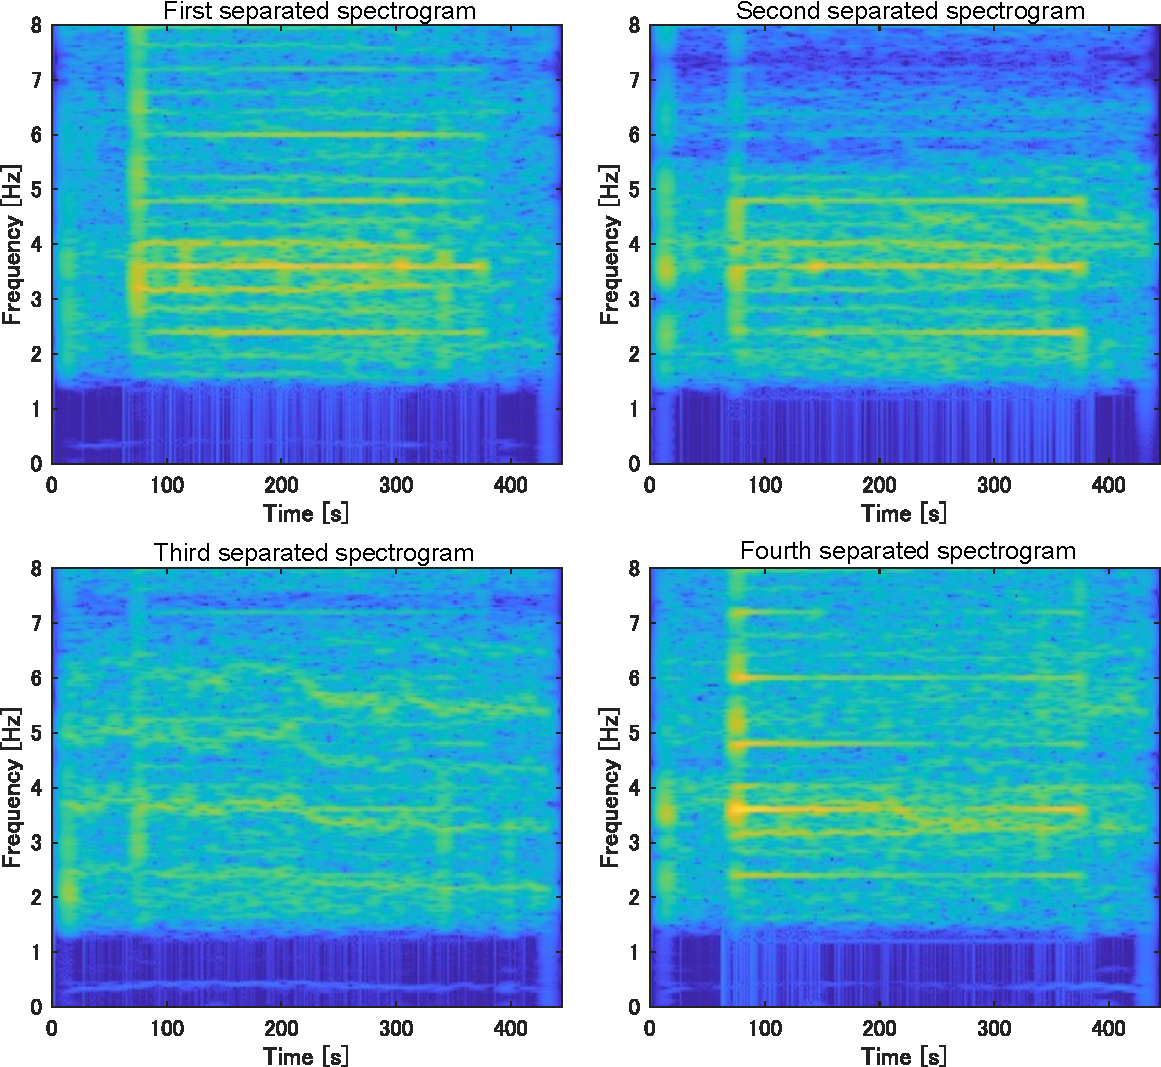
\includegraphics[width=1.0\hsize]{spect_iva_filter_64_est.pdf}
\vspace{-20pt} % 図とキャプション間の余白調整
\caption{Spectrograms of separated signal obtained by IVA (high-pass-filtered).}
\vspace{-15pt} % キャプション下部の余白調整
\label{fig:sfiva64est}
\end{figure}
%-%-%-%-%-%-%-%-%

%-%-%-%-%-%-%-%-%
\begin{figure}[tb]
\centering
\vspace{5pt} % 図上部の余白調整
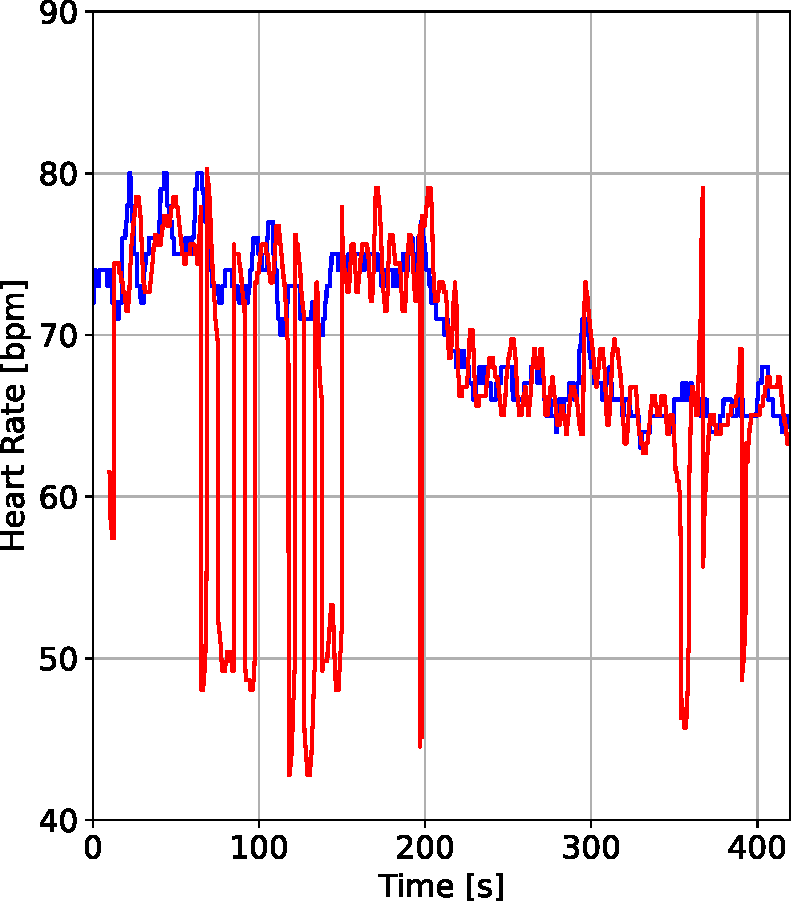
\includegraphics[width=50mm]{hr_iva_filter_64_ch3.pdf}
\vspace{-10pt} % 図とキャプション間の余白調整
\caption{Third Estimated (red) and reference (blue) heart rates obtained by IVA (high-pass-filtered).}
\vspace{-10pt} % キャプション下部の余白調整
\label{fig:fhriva64ch3}
\end{figure}
%-%-%-%-%-%-%-%-%

%----------------------------------------------
\subsubsection{ILRMAを適用した結果}
%----------------------------------------------
\hspace{1.0em}Fig. \ref{fig:silrma1}はフィルタを適用した観測信号にILRMAを適用した推定信号である.IVAの分離結果であるFig. \ref{fig:sfiva64est}では,1番目,2番目,及び4番目に心拍成分以外の成分が分離されていたが,Fig. \ref{fig:silrma1}では,振動成分が1番目及び4番目のスペクトログラムに分離され,2番目のスペクトログラムの4.5~Hz及び5.5~Hz付近に心拍成分がみられる.ここで,Fig. \ref{fig:sfiva64est}及びFig. \ref{fig:silrma1}の3番目のスペクトログラムを比較すると心拍成分のパワーに差がみられないことから,Fig. \ref{fig:sfiva64est}の3番目以外のスペクトログラムにも心拍成分が混在していたと考えられる.

また,Fig. \ref{fig:silrma1}に対して心拍推定アルゴリズムを適用した心拍推定値をFig. \ref{fig:hrilrma1}に示す.IVAを用いた際の推定心拍であるFig. \ref{fig:fhriva64ch3}では60~sから150~s及び360~sから400~sの推定心拍値が参照値と合致していなかったが,基底数固定型ILRMAでは60~sから120~s以外の時間で参照値とよく合致している.不一致の時間に関しては振動台の信号が加えられた初期であり,大きく体が動いたことが参照値と外れた原因と考えられる.

%-%-%-%-%-%-%-%-%
\begin{figure}[tb]
\centering
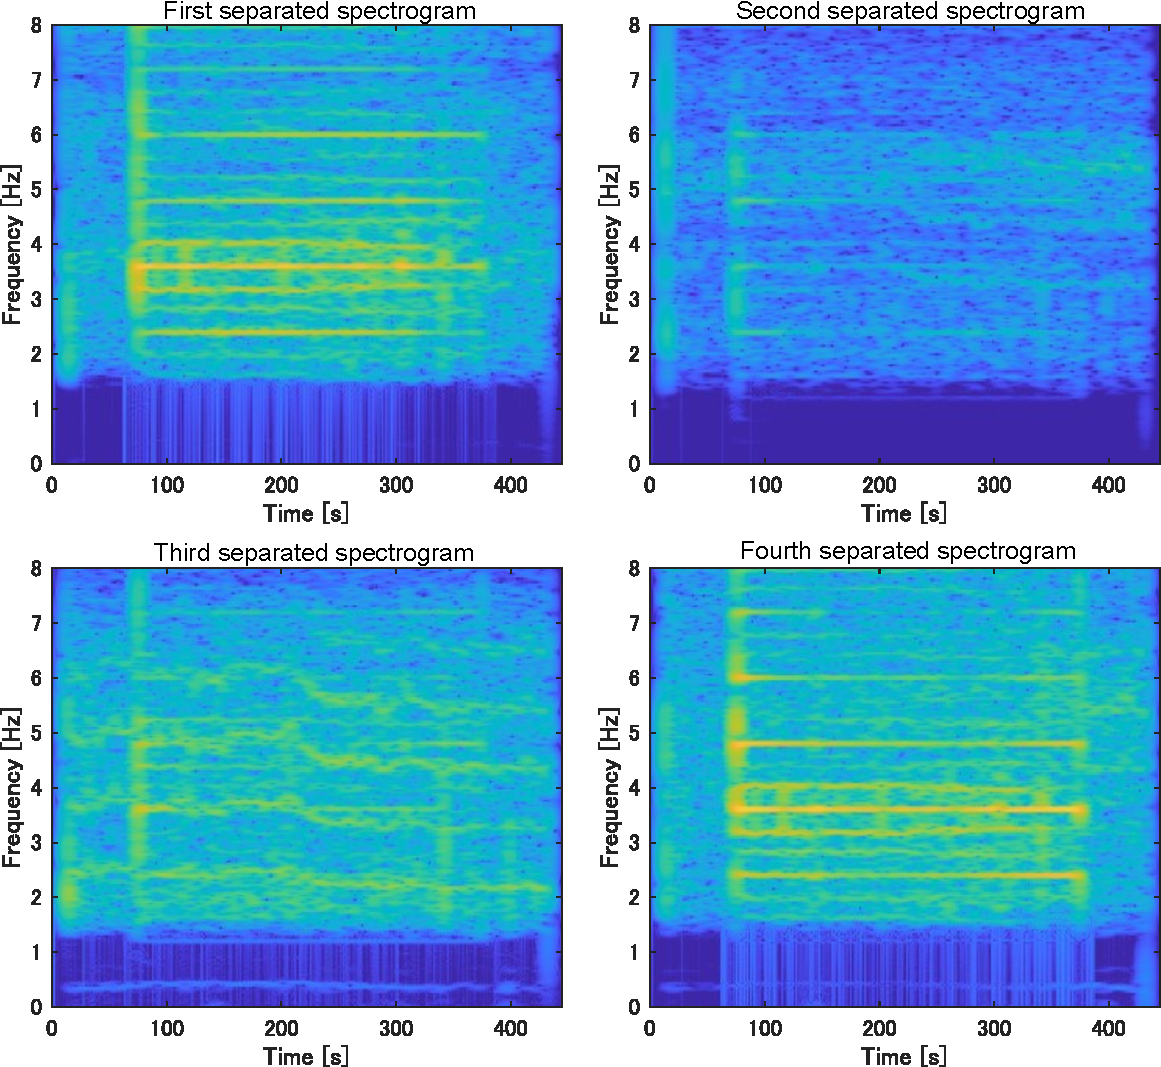
\includegraphics[width=1.0\hsize]{spect_ILRMA1_64_est.pdf}
\vspace{-20pt} % 図とキャプション間の余白調整
\caption{Spectrograms of separated signal obtained by ILRMA (high-pass-filtered).}
\vspace{-20pt} % キャプション下部の余白調整
\label{fig:silrma1}
\end{figure}
%-%-%-%-%-%-%-%-%

%-%-%-%-%-%-%-%-%
\begin{figure}[tb]
\centering
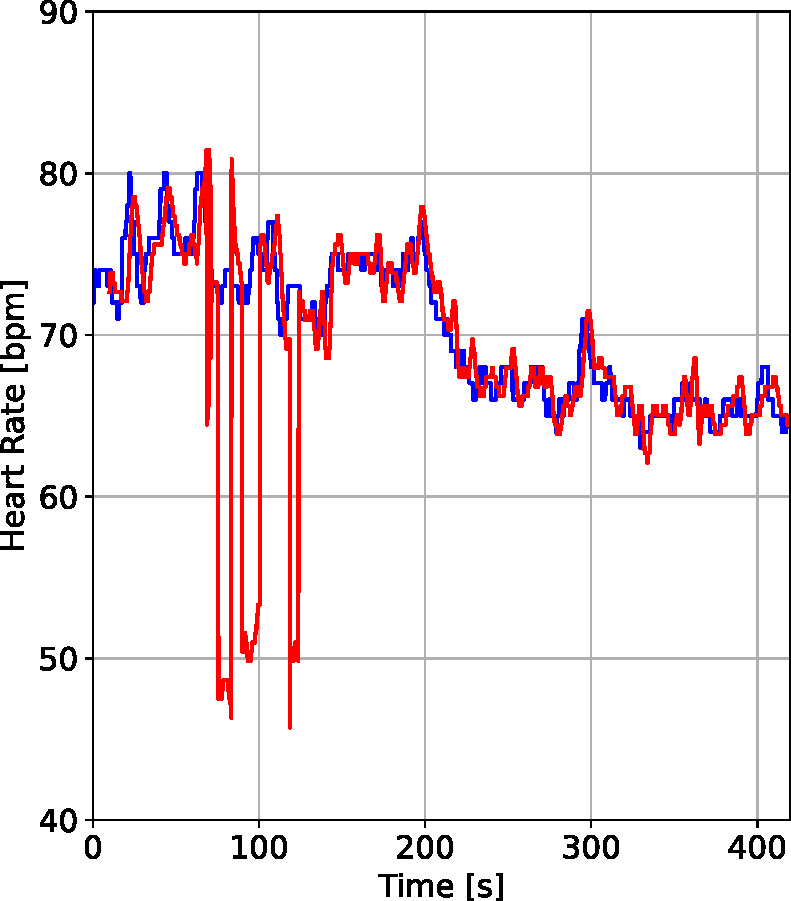
\includegraphics[width=50mm]{hr_ILRMAtype1_64_ch3.pdf}
\vspace{-10pt} % 図とキャプション間の余白調整
\caption{Third Estimated (red) and reference (blue) heart rates obtained by ILRMA (high-pass-filtered).}
\vspace{-10pt} % キャプション下部の余白調整
\label{fig:hrilrma1}
\end{figure}
%-%-%-%-%-%-%-%-%

%----------------------------------------------
\section{結論}
%----------------------------------------------
\hspace{1.0em}

\begin{comment}
\section{出筆上の簡単な注意点}
\hspace{1.0em}
詳細は執筆要項をご覧下さい。

\subsection{原稿}
\hspace{1.0em}
原稿はワープロ等を用いて{\bf A4サイズ}で作成して下さい.
原稿は{\bf 6枚以内}です.
6枚を越えた原稿は受け付けませんので,ご注意下さい.
\underline{\bf 上下のマージンは25mm以上,左右のマージンは}\\
\underline{\bf 17mm以上}にして下さい.\\
上記の余白には何も記述しないでください.たとえば,ページ番号などです.

\subsection{文字の色・大きさ・フォント}
\hspace{1.0em}
文字は黒色を用いて下さい.(カラーは不可)
目安として表題16ポイント、著者名・所属・本文10.5ポイント以上をお使い下さ
い。

\subsection{図と表,写真}
\hspace{1.0em}
図と表:直接原稿中に張り込んでください.

\section{原稿提出方法}
\hspace{1.0em}
\underline{\bf Web上から電子的に提出してください。}\\
(URL: %%WSURL)\\
なお、印刷・製本スケジュールの関係上,提出期限後の原稿訂正,差し替えには応
じかねますので,ご注意下さい.

\section{問い合わせ先}
出版担当幹事までお願いします。

\vspace{13em}
\end{comment}

\begin{thebibliography}{99}
\itemsep 1pt % 項目の間隔微調整用
\fontsize{8pt}{8pt}\selectfont  % 項目のフォントサイズ微調整用

\bibitem{originica}
P. Comon, "Independent component analysis, A new concept?," {\em Signal Processing}, vol. 36, no. 3, pp.287--314, 1994.

\bibitem{Kim2007_iva}
T.~Kim, H.~T.~Attias, S.-Y.~Lee, and T.-W.~Lee, ``Blind source separation exploiting higher-order frequency dependencies,'' 
{\em IEEE Trans. Audio, Speech, and Language Processing}, vol.~15, no.~1, pp.~70--79, 2007.

\bibitem{auxIVA}
N.~Ono and S.~Miyabe, ``Auxiliary-function-based independent component analysis for super-Gaussian sources,'' 
{\em Proc. International Conference on Latent Variable Analysis and Signal Separation,} pp.165--172, 2010.

\bibitem{ILRMA}
D.~Kitamura, N.~Ono, H.~Sawada, H.~Kameoka, and H.~Saruwatari,
``Determined blind source separation unifying independent vector analysis and nonnegative matrix factorization,'' 
{\em IEEE/ACM Trans. Audio, Speech, and Language Processing}, vol.~24, no.~9, pp.~1626--1641, 2016.

\bibitem{Kitamura2018_ilrma}
D.~Kitamura, N.~Ono, H.~Sawada, H.~Kameoka, and H.~Saruwatari, ``Determined blind source separation with independent low-rank matrix analysis,'' 
{\em Audio Source Separation}, S.~Makino, Ed., pp. 125--155. Springer, Cham, 2018.

\bibitem{permute}
S. Kurita, H. Saruwatari, S. Kajita, K. Takeda, and F. Itakura, ``Evaluation of blind signal separation method using directivity pattern under reverberant conditions,'' {\em Proc. International Conference on Acoustics, Speech, and Signal Processing}, vol. 5, pp. 3140--3143, 2000.

\bibitem{persolve1}
N. Murata, S. Ikeda, and A. Ziehe, ``An approach to blind source separation based on temporal structure of speech signals,'' {\em Neurocomputing}, vol. 41, no. 1--4, pp. 1--24, 2001.

\bibitem{persolve2}
H. Sawada, R. Mukai, S. Araki, and S. Makino, ``A robust and precise method for solving the permutation problem of frequency-domain blind source separation,'' {\em IEEE Trans. Speech Audio Process.}, vol. 12, no. 5, pp. 530--538, 2004.

\bibitem{persolve3}
H. Saruwatari, T. Kawamura, T. Nishikawa, A. Lee, and K. Shikano, ``Blind source separation based on a fast-convergence algorithm combining ICA and beamforming,'' {\em IEEE Trans. Audio, Speech, Lang. Process.}, vol. 14, no. 2, pp. 666--678, 2006.

\bibitem{persolve4}
H. Sawada, S. Araki, and S. Makino, ``Measuring dependence of bin-wise separated signals for permutation alignment in frequency-domain BSS,'' {\em Proc. IEEE Int. Symp. Circuits Syst.}, pp. 3247–3250, 2007.

\bibitem{auxfunc}
D.~R.~Hunter and K.~Lange, ``A tutorial on MM algorithms,'' 
{\em The American Statistician,} vol.~58, no.~1, pp.~30-–37, 2004.

\bibitem{stable_auxIVA}
N.~Ono,
``Stable and fast update rules for independent vector analysis based on auxiliary function technique,''
{\em Proc. IEEE Workshop on Applications of Signal Processing to Audio and Acoustics}, pp.189--192, 2011.

\bibitem{isnmf}
C.~Févotte, N.~Bertin, J.-L.~Durrieu, 
``Nonnegative matrix factorization with the Itakura-Saito divergence. With application to music analysis.'' 
{\em Neural Computation}, vol.~21, 793--830, 2009.

%\bibitem{abc} 著者名、``題目''
%{\em 出典論文誌名}, Vol. XX, No. YY, pp.ZZ1-ZZ2, Dec., 1996

%\bibitem{def} 著者名、``題目''
%{\em 出典論文誌名}, Vol. XX, No. YY, pp.ZZ1-ZZ2, Dec., 1996

\end{thebibliography}

\end{document}
